\documentclass[tikz, border=4mm]{standalone}
\usetikzlibrary{positioning,fit,calc}
\tikzstyle{line}=[draw]
\begin{document}
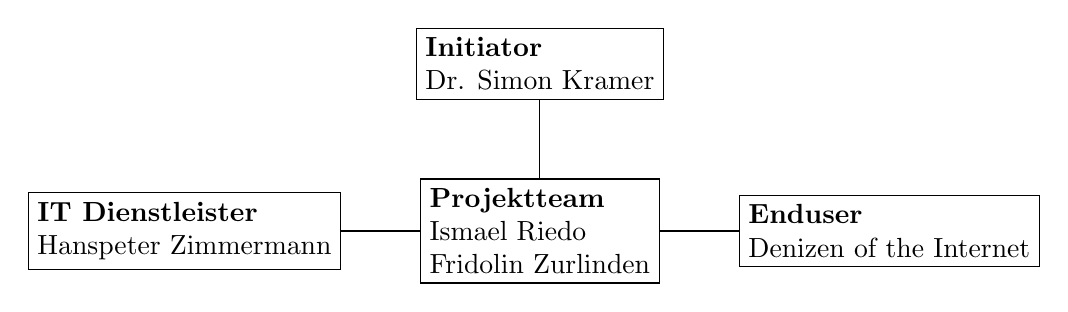
\begin{tikzpicture}
    \node[draw, align=left] (a) {\textbf{Initiator} \\ Dr. Simon Kramer};
    \node[draw, below=of a, align=left] (p) {\textbf{Projektteam} \\ Ismael Riedo \\ Fridolin Zurlinden};
    \node[draw, align=left, left=of p] (i) {\textbf{IT Dienstleister} \\ Hanspeter Zimmermann};
    \node[draw, align=left, right=of p] (e) {\textbf{Enduser} \\ Denizen of the Internet};
    \path[line] (p) -- (a);
    \path[line] (p) -- (i);
    \path[line] (p) -- (e);
\end{tikzpicture}
\end{document}
